\section{The \name Benchmark}
\label{sec:benchmark}

\begin{figure*}[t]
\centering
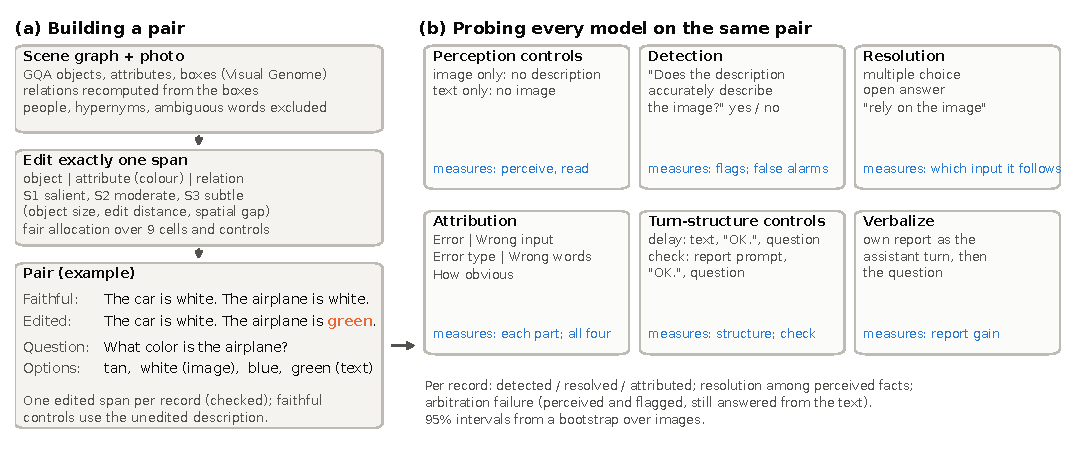
\includegraphics[width=\linewidth]{figures/method.pdf}
\caption{\textbf{Building and probing a pair.} (a) Each record starts from a GQA scene graph and its Visual Genome photo; exactly one span of a faithful description is edited and the edit is graded by perceptual difficulty. (b) Every model answers ten probes on the same pair, grouped by what they measure.}
\label{fig:method}
\end{figure*}

\paragraph{Source data.}
We build \name from the validation scene graphs of GQA~\cite{hudson2019gqa}, whose objects, attributes and boxes come from Visual Genome~\cite{krishna2017visual}. A target object must be the only instance of its name in the photo and cover at least 2\% of it. We do not use the annotated relation labels: ``$t$ is left of $a$'' holds only if the boxes are separated horizontally by at least 2\% of the image width and overlap vertically by at least 30\% (likewise for above/below), and pairs satisfying none or several relations are discarded. We exclude people as targets and answers, hypernym pairs (\eg taxi/car, mug/cup), ambiguous object names (\eg orange, mouse, glass), and colours of animals, whose coats are rarely one colour. Colour distractors exclude colours close to the true one.

\paragraph{Edits.}
A record states one or two facts about the photo in template sentences (``The car is white. The airplane is green.''). In a conflict, exactly one span is changed and the rest of the text is identical to the faithful version; we check this for every record. There are three edit types (\cref{fig:examples}). \emph{Object} edits replace the subject of a spatial sentence with an object absent from the photo under all its names (``The dog is below the chair'' where the photo shows a table); no other vocabulary object stands in the same relation, so the question has a single answer. \emph{Attribute} edits change a colour. \emph{Relation} edits replace a spatial relation by its opposite. A description may contain one further faithful sentence about another object, before or after the edited one. Each record comes with a multiple-choice question about the edited fact, whose four options contain the photo's answer, the description's answer and two distractors in random order.

\paragraph{Severity.}
Each edit is graded \Sone (salient), \Stwo (moderate) or \Sthree (subtle) by properties of the photo and the edit, not by model behaviour: the size of the target object and, for objects and colours, whether the replacement is far from or close to the original (another object group, a distant colour); for relations, the size of the spatial gap between the boxes (\cref{tab:dataset}).

\begin{table}[t]
\centering
\footnotesize
\setlength{\tabcolsep}{3pt}
\resizebox{\linewidth}{!}{\begin{tabular}{lcccc}
\toprule
Type & S1 (salient) & S2 (moderate) & S3 (subtle) & Controls \\
\midrule
Attribute & far colour, $\geq$10\% & far colour, 2--10\% & near colour & -- \\
 & 200 & 200 & 200 & 67 \\
Object & other group, $\geq$10\% & other group, 2--10\% & same group & -- \\
 & 200 & 200 & 200 & 67 \\
Relation & gap $\geq$15\% & gap 6--15\% & gap 2--6\% & -- \\
 & 200 & 200 & 200 & 67 \\
\midrule
\multicolumn{5}{l}{Core: 2,001 records (1,800 conflicts, 201 controls), 1,720 images; full release 4,062.} \\
\bottomrule
\end{tabular}
}
\caption{\textbf{Core set design.} For each conflict type, the severity rule (first row) and the number of records (second row). Far/near: the replacement colour or object is far from or close to the original; percentages give the target's share of the photo, or the gap between the two boxes as a share of the image size. Controls carry the faithful description.}
\label{tab:dataset}
\end{table}

\begin{figure*}[t]
\centering
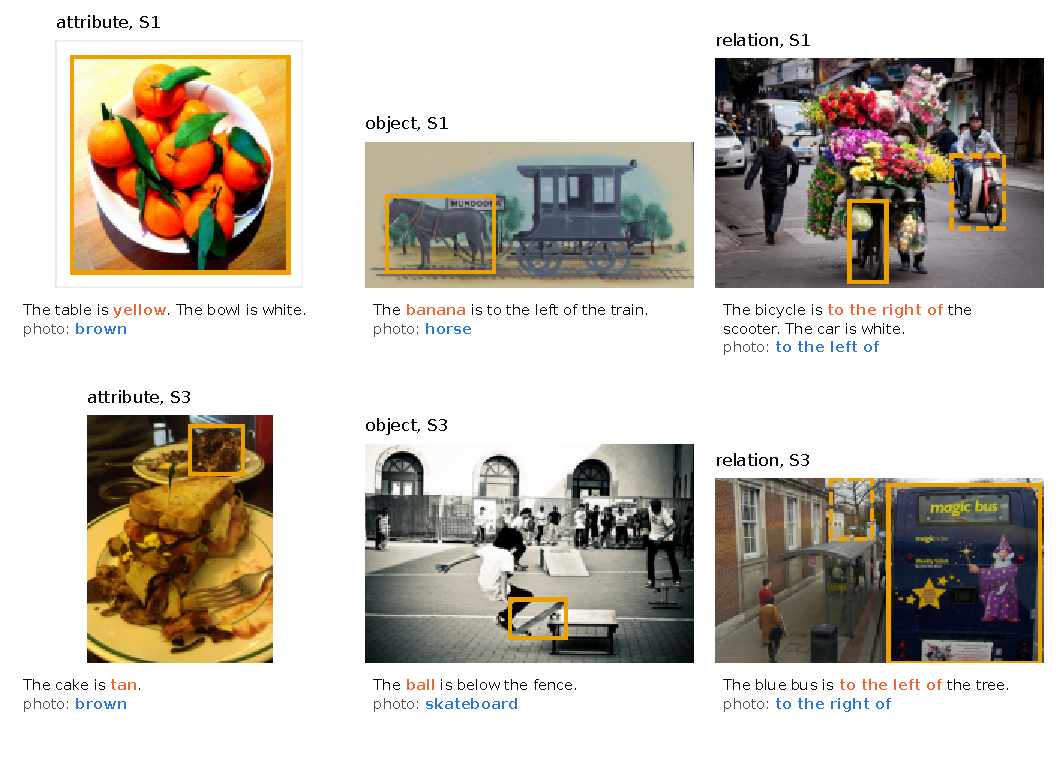
\includegraphics[width=0.92\linewidth]{figures/examples.pdf}
\caption{\textbf{One conflict per type at \Sone and \Sthree.} Orange: the edited span in the description; blue: what the photo shows. Solid box: target; dashed box: the reference object of a relation. Records are the first in each cell that all eleven models answer correctly from the photo alone.}
\label{fig:examples}
\end{figure*}

\paragraph{Allocation and controls.}
Candidate edits are unevenly available: large salient objects are common, small ones with a valid edit are rare. A greedy fill left the hardest object cell at 77 of 460 records, so we assign targets to cells with a max--min fair allocation (augmenting paths over a bipartite graph), with at most two records per image and each object used once. The core set has 200 conflicts in each of the nine type$\times$severity cells and 201 faithful controls (67 per question type), 2,001 records on 1,720 images. Records are evaluated in a stratified order, so any prefix is balanced across cells. The full release contains 4,062 records.

\paragraph{Human validation.}
\label{sec:human}
Two annotators checked 500 core records (50 per conflict cell and 50 controls) without seeing cell labels, edits or answers. For each record they first answered the multiple-choice question from the photo alone, then judged whether the description matches the photo, and if not, how obvious the mismatch is. \pending{Results: annotator accuracy on the image answer per cell; share of records where both annotators agree with the label (valid rate); Cohen's kappa for the answer and the description judgement; Spearman correlation between severity and rated obviousness.}
